\documentclass[table]{beamer}
\mode<presentation>
\usetheme{Berlin}
\usecolortheme{beaver}
\usepackage{listings}
\usepackage{multirow}

%%%
% TITLE PREAMBLE
\title[Intro to Bioinformatics] % (optional, only for long titles)
{An Introduction to Bioinformatics Tools}
\subtitle{Part 2: BLAST}
\author[Pritchard, Cock] % (optional, for multiple authors)
{Leighton~Pritchard \and Peter~Cock}
\institute[The James Hutton Institute] % (optional)
{
  Information and Computational Sciences\\
  The James Hutton Institute
}
\date[May 2014] % (optional)
{Bioinformatics Training, 29$^{th}$,30$^{th}$ May 2014}
\subject{Bioinformatics}

%%%
% TOC
% Show table of contents, with current section highlighted,
% at the start of each section
\AtBeginSection[]
{
  \begin{frame}
    \frametitle{Table of Contents}
    \tableofcontents[currentsection]
  \end{frame}
}


%%%
% START DOCUMENT
\begin{document}

  \frame[plain]{\titlepage}
  
%%%
% SECTION: BLAST Essentials
  \section{BLAST Essentials}
  
    % What is BLAST
    \subsection{What is BLAST?}
    \begin{frame}
     \frametitle{What BLAST Is}
     \begin{itemize}
       \item<1-> BLAST:
       \begin{itemize}
         \item<1-> Basic (it's actually sophisticated)
         \item<1-> Local Alignment (what it does: local sequence alignment)
         \item<1-> Search Tool (what it does: search against a database)
       \end{itemize}
       \item<2-> The most important software package in bioinformatics?
       \item<2-> Fast, robust, sequence similarity search tool
       \item<2-> Not foolproof.
     \end{itemize}
    \end{frame}
  
    \begin{frame}
     \frametitle{What A BLAST Search Is}
     \begin{itemize}
       \item BLAST search = identification of similar sequences in a database
       \item This depends on:
       \begin{itemize}
         \item query sequence
         \item BLAST program (and choice of BLAST/BLAST+, version No.)
         \item database
         \item search parameters
       \end{itemize}
     \end{itemize}
    \end{frame}  
  
    % Sequence Alignment
    \subsection{Sequence Alignment}
    \begin{frame}
     \frametitle{Assumptions}
     You are familiar with
     \begin{itemize}
       \item biological sequences (RNA, DNA, protein)
       \item mutation, drift, molecular clocks
       \item gene and genome structure (including repeats, pseudogenes etc.)
       \item homology, paralogy, orthology, etc.
     \end{itemize}
     - all important for interpretation of BLAST output
    \end{frame}

    \begin{frame}
     \frametitle{Alignment Search Space}
     Consider two biological sequences to be aligned$\ldots$
     \begin{itemize}
       \item One sequence on the \textit{x}-axis, the other on the \textit{y}-axis
       \item Each point in space is a pairing of two letters
       \item Ungapped alignments are diagonal lines in the search space, gapped alignments have short 'breaks'
       \item There may be one or more "optimal" alignments
     \end{itemize}
     \begin{center}
       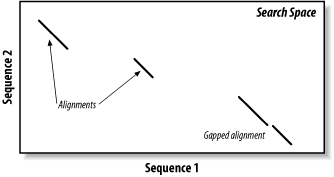
\includegraphics[width=0.4\textwidth]{images/search_space} 
     \end{center}
   \end{frame}
    
    \begin{frame}
     \frametitle{Global \textit{vs} Local Alignment}
     \begin{itemize}
       \item<1-> Global alignment: sequences are aligned along their entire lengths
       \item<1-> Local alignment: the best subsequence alignment is found
       \item<2-> Consider an alignment of the same gene from two distantly-related eukaryotes, where:
         \begin{itemize}
           \item<2-> Exons are conserved and small in relation to gene locus size
           \item<2-> Introns are not well-conserved but large in relation to gene locus size
         \end{itemize}
       \item<3-> Local alignment will align the conserved exon regions
       \item<3-> Global alignment will align the whole (mostly unrelated) locus
     \end{itemize}
    \end{frame}

    % dynamic programming
	\subsubsection{Dynamic Programming}
    \begin{frame}
     \frametitle{Dynamic Programming}
     \begin{itemize}
       \item<1-> We aim to align the words
       \begin{itemize}
         \item<1-> \texttt{COELACANTH}
         \item<1-> \texttt{PELICAN}
       \end{itemize}
       \item<2-> Each identical letter (match) scores +1
       \item<2-> Each different letter (mismatch) scores -1
       \item<2-> Each gap scores -1
       \item<3-> \emph{Alignment is maximisation of the alignment score}
     \end{itemize}
    \end{frame}   
   
    \begin{frame}
     \frametitle{Dynamic Programming}
     \framesubtitle{Initialise the matrix}
       \begin{center}
         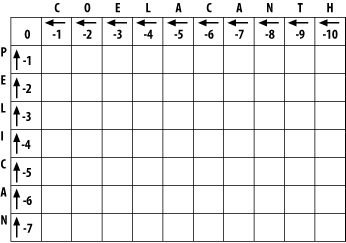
\includegraphics[width=0.5\textwidth]{images/initialise}
       \end{center}
    \end{frame}   
   
    \begin{frame}
     \frametitle{Dynamic Programming}
     \framesubtitle{Fill the cells}
       \begin{center}
         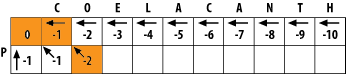
\includegraphics[width=0.5\textwidth]{images/fill_start} \\
         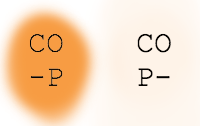
\includegraphics[width=0.3\textwidth]{images/fill_start_letters}
       \end{center}
    \end{frame}     

    \begin{frame}
     \frametitle{Dynamic Programming}
     \framesubtitle{Fill the matrix}
       \begin{center}
         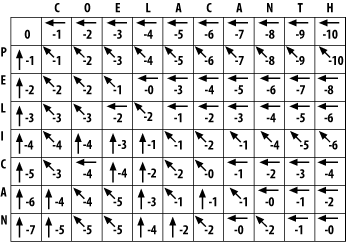
\includegraphics[width=0.5\textwidth]{images/full_matrix}
       \end{center}
       Matrix represents all possible pairwise alignments and scores
    \end{frame}  
   
    \begin{frame}
     \frametitle{Dynamic Programming}
     \framesubtitle{Traceback}
       \begin{center}
         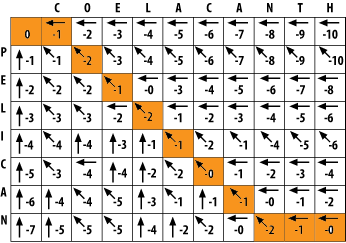
\includegraphics[width=0.5\textwidth]{images/traceback} \\
         
\includegraphics[width=0.3\textwidth]{images/traceback_sequence}         
       \end{center}
    \end{frame}     

    \begin{frame}
     \frametitle{Dynamic Programming}
     \framesubtitle{Algorithms}
       \begin{itemize}
         \item<1-> Global: Needleman-Wunsch (as in example)
         \item<1-> Local: Smith-Waterman (differs from example)
         \item<2-> NW/SW are \emph{guaranteed} to find the optimal match \emph{with respect to the scoring system being used}: a model parameter.
         \item<2-> Alignment is an approximation: no scoring scheme encapsulates biological "truth"
         \item<2-> Any pair of sequences can be aligned: finding meaning is up to you
       \end{itemize}
    \end{frame}   

    \begin{frame}
     \frametitle{Dynamic Programming}
     \framesubtitle{Gap Scoring}
       \begin{itemize}
         \item Simple gap penalty: all gaps score the same
         \begin{itemize}
           \item \emph{one} parameter in the alignment model
         \end{itemize}
         \item Affine gap penalty: opening and extending score differently
         \begin{itemize}
           \item \emph{two} parameters in the alignment model
         \end{itemize}
       \end{itemize}
       \begin{center}
         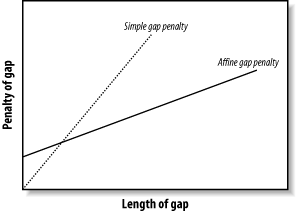
\includegraphics[width=0.3\textwidth]{images/gap_scores} 
       \end{center}
     \end{frame}  
   
    \begin{frame}
     \frametitle{Dynamic Programming}
     \framesubtitle{Banded Alignment}
       \begin{itemize}
         \item Given a maximum scoring alignment, restrict search to a "band" between endpoints
         \item Width of this band = "bandwidth", another parameter in the model
         \item Speeds up search, reduces memory use
       \end{itemize}
       \begin{center}
         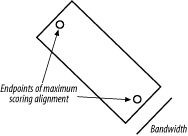
\includegraphics[width=0.3\textwidth]{images/banded} 
       \end{center}
     \end{frame}     


    % The BLAST Algorithm
    \subsection{The BLAST Algorithm}
    \begin{frame}
     \frametitle{BLAST Is A Heuristic}
     \begin{itemize}
       \item<1-> BLAST does not use Needleman-Wunsch or Smith-Waterman
       \item<1-> BLAST \emph{approximates} dynamic programming methods
       \item<1-> BLAST is not guaranteed to give an optimal alignment (for chosen parameters)
       \item<2-> BLAST does not explore the complete search space
       \item<3-> BLAST uses heuristics (loosely-defined rules) to refine High Scoring Pairs
       \item<4-> BLAST reports "statistically-significant" alignments (dependent on parameters)
     \end{itemize}
   \end{frame}

  \begin{frame}
    \frametitle{Steps in the Algorithm}
    \begin{enumerate}
      \item Seeding
      \item Extension
      \item Evaluation
    \end{enumerate}
  \end{frame}

  % seeding
  \begin{frame}
    \frametitle{About BLAST databases$\ldots$}
    \begin{itemize}
      \item The database used is a parameter in your model
      \item Three components:
      \begin{itemize}
        \item header file: \texttt{*.phr}, \texttt{*.nhr}
        \item sequence file: \texttt{*.psq}, \texttt{*.nsq}
        \item index file: \texttt{*.pin}, \texttt{*.nin}
      \end{itemize}
      \item The index allows for fast searching                
    \end{itemize}
  \end{frame}
  
  \begin{frame}
    \frametitle{About BLAST databases$\ldots$}
    \begin{itemize}
      \item The database used is a parameter in your model
      \item Three components:
      \begin{itemize}
        \item header file: \texttt{*.phr}, \texttt{*.nhr}
        \item sequence file: \texttt{*.psq}, \texttt{*.nsq}
        \item index file: \texttt{*.pin}, \texttt{*.nin}
      \end{itemize}
      \item The index allows for fast searching                
    \end{itemize}
  \end{frame}

  % seeding
  \subsubsection{Seeding}
  \begin{frame}
    \frametitle{Word Hit}
    \begin{itemize}
      \item A short sequence and its \emph{neighbourhood}
      \item \emph{neighbourhood}: words of same length whose aligned score is less than a threshold value $T$
      \item Three parameters: scoring matrix, word size $W$, and $T$
    \end{itemize}
    \begin{center}
      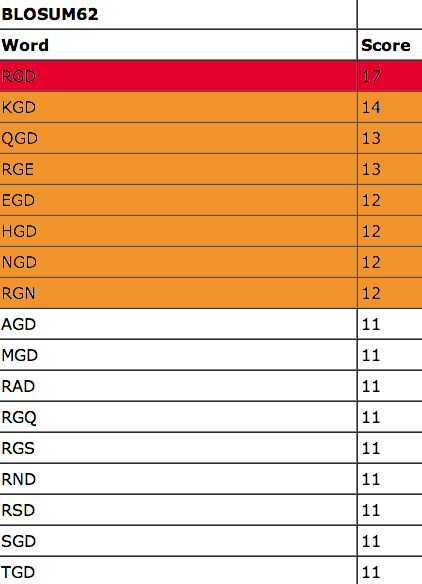
\includegraphics[width=0.3\textwidth]{images/neighbourhood} 
    \end{center}    
  \end{frame}

  \begin{frame}
    \frametitle{Seeding}
    \begin{itemize}
      \item BLAST assumption: significant alignments have \emph{words} in common
      \item BLAST finds word (\emph{neighbourhood}) hits in the database index
      \item Word hits are used to \textit{seed} alignments
    \end{itemize}
    \begin{center}
      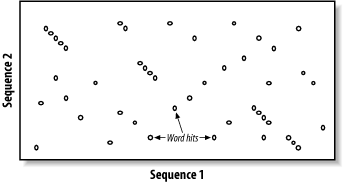
\includegraphics[width=0.5\textwidth]{images/seeding} 
    \end{center}    
  \end{frame}

  \begin{frame}
    \frametitle{Seeding Controls Sensitivity}
    \begin{itemize}
      \item Word size $W$ controls number of hits (smaller words $\implies$ more hits)
      \item Threshold score $T$ controls number of hits (lower threshold $\implies$ more hits)
      \item Scoring matrix controls which words match
    \end{itemize}
    \begin{center}
      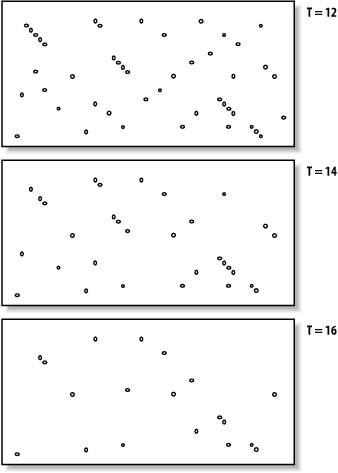
\includegraphics[width=0.25\textwidth]{images/seeding_t} 
    \end{center}    
  \end{frame}

  \begin{frame}
    \frametitle{The Two-Hit Algorithm}
    \begin{itemize}
      \item BLAST assumption: word hits cluster on the diagonal for significant alignments
      \item The acceptable distance between words on the diagonal $A$ is a parameter of your model
      \item Smaller distances isolate single words, and reduce search space
    \end{itemize}
    \begin{center}
      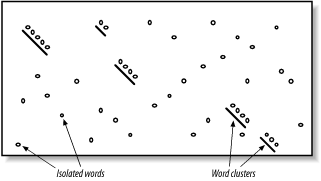
\includegraphics[width=0.5\textwidth]{images/two_hit} 
    \end{center}    
  \end{frame}


  
  % Using BLAST   
  \section{Using BLAST}
    \subsection{Which BLAST tool should I use?}
    \begin{frame}
     \frametitle{}
    \end{frame}

    \subsection{Controlling BLAST output}
    \begin{frame}
     \frametitle{}
    \end{frame}
     
    \subsection{Interpreting BLAST output}
    \begin{frame}
     \frametitle{}
    \end{frame}
    
% etc
\end{document}